\documentclass[./Main.tex]{subfiles} 
\begin{document}

\section{Geo-location-attempt }
\subsection{Introduction}

While the foundation of all calculations in a regional word attempt is a manually created list of only a few hundred words along with their probability distribiutions, we first wanted to try using machine learning techniques to generate such list automatically.

Although the manually created list and its values are based on scientific research, it could mark the weak spot of the regional word attempt for number of reasons. For example people in a specific region could use a typical word in their everyday language while speaking to their friends and family, but it is not quite sure that they also use this words in their written language, even if it is only their private Twitter account. In addition, the list is way too short to cover only fraction of the words people use on Twitter, so the end results mostly rely on the data that is generated during the main algorithm's loops.

It seemed we had no other choice but to trust this generated values, so we came up with the idea of first skipping the manually created word list and use an automatically created one -- based on a corpus of geo annotated Tweets instead.

Before entering the main loop, we had to write an algorithm that learns the distribution in all seven regions for all the words in the corpus. This way we are generating a list that covers a very huge percentage of all words that could occur in a Tweet.

We struggled to find a good solution for representing the regions in a way that would allow us to easily check from which of them a geo annotated Tweet was sent. After a few unsuccessful approaches we decided to define polygons for the regions that neither are overlapping each other nor leave gaps between them. For the value of the points we simply used their longitude and latitude coordinates, which can be represented as floating point numbers.

\begin{figure}
  \begin{center}
   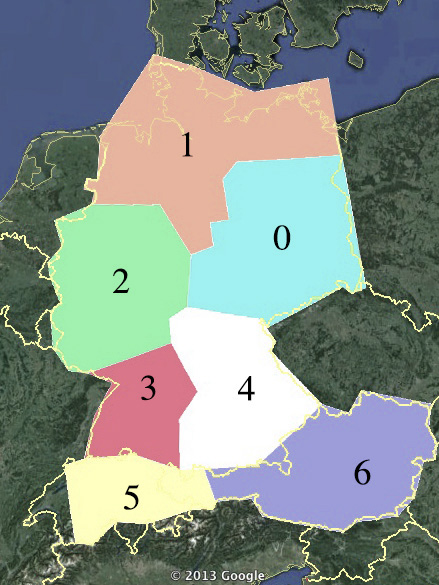
\includegraphics[width=0.5\columnwidth]{../img/polygone_satt.jpg}
    \caption{\label{geo_polymap} Map of the regions and the index of their feature used in the vectors represented as polygons}
  \end{center}
\end{figure}

We did not implement a point-in-polygon algorithm ourself, but used the version of Joel Lawhead published on geospatialpython.com \cite{GeoPy} instead.  
To find out where a Tweet was sent from, we iterate over all regions and return the first one, where the point-in-polygon function returns true.
In this first step, the tweet-vector starts with the value 0 for all features, except the one standing for the region of origin, which we assign the value 1 to.

\begin{algorithm}[t]
 \SetAlgoLined
 \KwData{\\
	$tweets$: Corpus of geo-annotated documents\\ 
	$stopwords$: List of stopwords}
 \KwResult{\\$WV$: normalized word-vectors, representing\\ the probability distribiution for each word}
 $WV \gets\emptyset $\; 
\ForEach{\label{alg:goto}tweet in tweets}{
$region \gets \texttt{Classify(}tweet\texttt{)}$\;
 $\vec{tweet} \gets \texttt{CreateVector(}region\texttt{)}$\;
 \ForAll{token in tweet}{
  \If{token $\notin$ stopwords}{
     $WV(token) \gets WV(token) + \vec{tweet} $\;
   }
}
}
 \ForEach{$\vec{word}$ in $WV$}{
$\vec{word} \gets$ \texttt{normalize(}$\vec{word}$\texttt{)}\;
}
\Return $WV$\;
\label{geo-algo}
\caption{Geo-algorithm}
\end{algorithm}

Let us assume that the coordinates of some Tweet reveal that its region is \textit{Westdeutschland,} represented by the feature with the index $3$.
Therefore the tweet-vector is $(0,0,1,0,0,0,0)$. 
The next step consists in iterating over all tokens in the Tweet and add the tweet-vector to their according word-vectors. To put it simply, we increase the counter for the specific feature of all occurring tokens by one. 
In the final step we iterate over all word-vectors and use our \texttt{normalize()}-function to attain the probability distribution showing how likely it is that the token is used in a specific region. By this normalization we make sure the format of the outcome is comparable to the initial list of the regional-word attempt and we can use it in the main algorithm without any adjustments.

\begin{figure}
\centering $\textrm{Example Tweet: } d = \textrm{'Hello Twitter!'} \textrm{ from the region 'Westdeutschland'.}$
 \begin{align*}
    \vec{t}_{hello} &= (1,3,2,5,2,1,0) \\
     \vec{t}_{twitter} &= (0,0,0,0,0,0,0) \\
      \vec{d} &= (0,0,1,0,0,0,0) \\
     \vec{t}_{hello}' &= \vec{t}_{hello} + \vec{d} =  (1,3,3,5,2,1,0) \\
    \vec{t}_{twitter} ' &= \vec{t}_{twitter} + \vec{d} = (0,0,1,0,0,0,0) \\
     \texttt{normalize(}\vec{t}'_{hello}\texttt{)} &= (0.04, 0.13, 0.13, 0.22, 0009, 0.04, 0) \\
     \texttt{normalize(}\vec{t}'_{twitter}\texttt{)} &= (0,0,1,0,0,0,0)
  \end{align*}
  \caption{Example for the creation of the initial word-vectors}
  \label{geo_example1}
\end{figure}

\subsection{Source of data}
The datasets used for the generation of the first word-vectors have been extracted from the Scheffler-corpus using the same classification function as described before. Although the corpus mostly consists of German Tweets (filtered with \emph{LangID}), about 20\% of the Tweets with geo-location have not been sent from one of the defined regions and therefore have been ignored. In addition, we filtered Retweets, Hashtags for the location-based social network 'Foursquare' (\emph{\#4sq} and \emph{\#foursquare}) as well as Hashtags from automatically sent messages and blocked the UserIDs for a few very frequent bots, that transfer their geo-location. The remaining data consists almost exclusively of German human-composed Tweets (although a very few English Tweets have remained in the corpus).

We created balanced sets, where the amount of Tweets are the same for all regions. As the fewest Tweets came from the region 6, \textit{Österreich} (8,787), we ended up with only 61,509 Tweets for all regions.  
In order to create a gold-standard, we subtracted 150 Tweets from each region, leaving us 60,459 for the training process.

Our assumption was that datasets of different sizes lead to different results, and we wondered in what way it would affect the accuracy to use the same data for the creation of the word-vectors in the geo-algorithm as we did for the main-algorithm. Therefore we created three balanced sets, one unbalanced set of all geo annotated Tweets and as a reference one huge set of unfiltered normal Tweets. Of course none of these sets do contain any Tweets from the gold-standard.
\begin{enumerate}
\item \emph{balanced-21k} with 3,000 Tweets from each region.
\item \emph{balanced-39k} consisting of the remaining 39,456 Tweets
\item \emph{balanced-61k} combining the both previous sets. 
\item \emph{geo-175k} with all Tweets from the corpus that were sent from one of the defined regions. Not balanced.
\item \emph{all-1500k} contains 1.5 million mostly not geo annotated Tweets.
\end{enumerate}
\subsection{Experiments}
As the algorithms leave us five parameters to alter, we had to run a series of experiments to find the optimal value for them. In the following we present our procedure and the results.

\subsubsection{Dataset combinations}
\label{dataset_section}
\begin{table}[b]
    \begin{tabular}{|l|lllll|}
    \hline
    Geo dataset     & balanced-21k & balanced-39k & balanced-61k & geo-175k & all-1500k \\ \hline
    balanced-21k    & 0.319        & 0.308        & 0.304        & 0.307           & 0.308       \\
    balanced-39k    & 0.306        & 0.353       & \textbf{0.345}        & \textbf{0.368 }          & 0.306       \\
    balanced-61k    & \textbf{0.336}        & \textbf{0.361}        & 0.344        &0.360           & 0.332       \\
    unbalanced-175k & 0.303        & 0.343        & 0.322        & 0.352           & \textbf{0.340}       \\ \hline
    \end{tabular} \\

  Calculation method: \textit{Normalized}; Stopwords: \textit{Top 200}; Loops: \textit{1}; Guessed amount of non-regional Tweets: \textit{60\%}, leading to a similarity threshold between \textit{0.999} and \textit{0.991}, depending on the dataset.
  \caption{Comparison of the combination of all datasets}
  \label{geo_datasets}
\end{table}

In order to give a solid foundation which data we should use in further experiments, we started to compare the combination of the five datasets we created. We wondered in what way it would affect the accuracy if we trained for instance the geo-algorithm with a small set of geo-annotated data but used a very big set of Tweets for the learning of the word-vectors in the loop of the main-algorithm. Another question was what results we would get if the data in the main-algorithm contained Tweets that had been used in the geo-algorithm before. 

Our expectation was in general that the accuracy would rise the more data we used and that the reuse of Tweets in the main-algorithm would lower it, because this data already had an effect and using it again would cause any change.

Unsurprisingly, using the smallest set, \emph{balanced-21k}, for the training of the geo-algorithm nearly always produced the lowest accuracy. 
But our hypothesis about the reuse of data was disproved: The combination of the \emph{balanced-39k} set for the learning in the geo-algorithm and \emph{balanced-61k} for the main-algorithm generated the third best result with an accuracy of 0.345.

We also discovered that the use of balanced data in the geo-algorithm, where all regions are represented by the same amount of documents, is crucial for good results. Having a look at the row for the \emph{unbalanced-175k}, it produces a very bad accuracy. Even in combination with the set containing 1.5 million Tweets \emph{(all-1500k),} it marks the second last rank.

This experiment showed us that we should use the \emph{balanced-39k}-set for the training of the geo-algorithm and the \emph{geo-175k}-set for the main-algorithm, because it generated the best accuracy of 0.365. We were surprised that the combination \emph{balanced-39k}/\emph{all-1500k} had a worse result, but interpreted it as a result of the unfiltered data of the \emph{all-1500k}-set.

\subsubsection{Comparison of different stopword-lists}
\begin{figure}[!b]
\begin{center}
\begin{tikzpicture}
        \begin{axis}[
                              width=0.9\columnwidth,
                              height=0.3\textheight,
                              symbolic x coords={0, 100, 200, 500, 750, 1000},
                              xtick=data,
                              ytick={0.28, 0.31, 0.34, 0.37},
			  ymax = 0.39,
                              ylabel=accuracy,
                              bar width=40,
                              xlabel=number of stopwords,
		 	 nodes near coords,
    			  nodes near coords align={vertical}
          ]
            \addplot[ybar,  postaction={ pattern=north west lines   }] coordinates {
               (0, 0.2762)
               (100, 0.352)
               (200, 0.368)
	      (500, 0.333)
               (750, 	0.318)
               (1000, 0.299)
            };
        \end{axis}
    \end{tikzpicture}
\end{center}

Calculation method: \textit{Normalized}; Geo-dataset: \textit{balanced-39k}, Main-dataset: \textit{geo-175k}; Loops: \textit{1}; Guessed amount of regional Tweets: \textit{60\%}
  \label{geo_graph1}
  \caption{Accuracy of different stopword-lists.}
  \label{geo_graph1}

\end{figure}

Zipf's law tells us that a very small amount of tokens are found extremely often in corpora, while most tokens appear only a few times. As it is much more likely for a more seldom word to have a regional meaning, we decided to filter out the most frequent token. 

We came up with the idea that it is not reasonable to use an existing stopword-list for the German language because people on Twitter could use specific words and symbols more often than in a standard German text. In addition, Tweets from spam bots or automatically sent messages that always contain the same words disturb the statistics and have to be filtered. So we used the Scheffler-corpus to create our own stopword-list using our modified version of Christopher Potts' tokenizer and counting the frequency of all tokens.

We were unsure about how many token should appear on a stopword-list, so we created five of them, containing the most \emph{100}, \emph{200}, \emph{500}, \emph{750} and \emph{1000} frequent words. Actually, we expected to have a better accuracy the more stopwords we use, but it turned out to be different.

Figure \ref{geo_graph1} shows clearly that more than 200 stopwords lead to worse results, probably because these words do have a regional meaning. On the other hand, only 100 stopwords have a lower accuracy than the list containing 200 entries. The fact, that the results of the run with no stopword filtering at all had the lowest accuracy, reveals the importance of using a stopword-list in general.

As the list containing 200 stopwords leads to the best accuracy of 0.37, we used this one in further experiments.

\subsubsection{Guessing the amount of regional Tweets}
 \label{geo_guessing}
\begin{figure}[!b]
\begin{tikzpicture}
       \pgfplotstableread{../data/geo_cos.csv}\data
       \begin{axis}[
           legend pos=south east,
           ylabel near ticks,
           axis y line*=left,
           xmin = 5,
           xmax = 100,
           ylabel= accuracy,
           xlabel= guessed percentage of non-regional Tweets,
           xtick = {5,10,20,30,40,50,60,70,80,90,100},
           width=0.9\columnwidth,
           height=0.5\textheight]
           \addplot[blue, mark=x] 
           table[x=Guess,y=Accuracy]{\data} ;
           \addlegendentry[font=\tiny]{accuracy}
       \end{axis}
       \begin{axis}[
           hide x axis,
           xmin = 5,
           xmax = 100,
           axis y line*=right,
           legend pos=south west,
           ylabel near ticks,
           ylabel= cosine similarity threshold,
           width=0.9\columnwidth,
           height=0.5\textheight]
           \addplot[red, mark=x] 
           table[x=Guess,y=Threshold]{\data};
           \addlegendentry[font=\tiny]{threshold}
       \end{axis}
\end{tikzpicture}
Calculation method: \textit{Normalized}; Geo-dataset: \textit{balanced-39k}, Main-dataset: \textit{geo-175k}; Stopwords: \textit{Top 200}; Loops: \textit{1}; 

  \caption{Relation between the amount of regional Tweets and the accuracy.}
  \label{geo_graph2}
\end{figure}
In section 2, \textit{Algorithms} we talked about the advantages and disadvantages of filtering too ordinary Tweets using the cosine similarity metric. Summarized, we gain much better results considering the accuracy, but have to accept that we cannot classify a huge percentage of Tweets because they do not differ enough from the average tweet-vector.

We wanted to know what accuracy we could achieve, so we ran the program a few times, changing the parameter guessing the amount of regional Tweets. We started at 100\% with no filtering at all and went down to an extreme of 5\%.

As figure \ref{geo_graph2} illustrates, the results approved our hypothesis that the accuracy rises, the lower we guess. At the same time the similarity threshold lowers to values of 0.92 at a guess of 5\%, showing that even these documents are very similar to the average tweet-vector.

The highest accuracy we could achieve had a value of 0.506, guessing that only 20\% of all Tweets are regional salient. We were extremely happy about this result, because we had an accuracy lower than 0.2, when we started our first experiments in the regional-word attempt. Nevertheless, we have to keep in mind that 80\% of all Tweet will be ignored, so for the majority of inputted Tweets we will not get any other results than that it is most likely written in standard German.

If we lower our guessing to 10\% or 5\%, the accuracy lowers again, probably because there are not enough Tweets left in the gold-standard to give a trustworthy result.

There is no ideal value for this parameter and eventually, people who will use this algorithm have to figure it out themselves, according to what they want to achieve: A higher coverage of data or a more reliable result. In the experiments to come, we decided to use a guessing of 20\%, because our aim is to achieve the highest possible accuracy.

\subsubsection{The right amount of loops}


The idea behind the loops in the main-algorithm was to estimate the probability distinction from which region a Tweet could have been sent from as many words as possible. Especially for the regional-list attempt this was a crucial approach to prevent the sparse data problem.

In this attempt on the other hand, this problem is not urgent, because we create a very large list of word-vectors based on a geo-annotated corpus. Therefore we asked ourselves, which amount of loops would lead to the best results. The more the better or the opposite? 

To find an answer to this question, we took the parameters we had proven to be the best choice in the experiments before, but varied the value for the loop-parameter from 0 to 20 and measured the accuracy. 
We were a bit puzzled to find out, that the main loop, even if it was only entered one time, lowers the accuracy by 0.023. Our new record for the accuracy becomes 0.53, if we chose a value of 0. Please keep in mind, that even though we do not enter the loop, the calculation of the word-vectors is always performed one time before that.

\begin{figure}[h]
\begin{tikzpicture}
       \pgfplotstableread{../data/geo_loops.csv}\data
       \begin{axis}[
           legend pos=south east,
           ylabel near ticks,
           xmin = 0,
           xmax = 20,
           ylabel= accuracy,
           xlabel= loops,
           xtick = {0,1,2,3,4,5,10,15,20},
           width=0.9\columnwidth,
           height=0.4\textheight]
           \addplot[blue, mark=x] 
           table[x=Loops,y=Accuracy]{\data} ;
       \end{axis}
\end{tikzpicture}
Calculation method: \textit{Normalized}; Geo-dataset: \textit{balanced-39k}, Main-dataset: \textit{geo-175k}; Stopwords: \textit{Top 200}; Guessed amount of regional Tweets: \textit{20\%}
  \caption{Amount of loops in the algorithm and their effect on the accuracy.}
  \label{geo_graph3}
\end{figure}

If we have a look at the graph in figure \ref{geo_graph3}, we can see clearly  that the accuracy drastically decreases, the more loops we enter. So our assumption, that the loops in the main-algorithm would lead to better results has been falsified. We then came up with the explanation, that the more often we use a loop, the more do all word-vectors approach an average vector and in this way lose all signs of a specific region.

Since the importance of the dataset for the main-algorithm drops, if we choose not to use the loop, we repeated the experiment in section \ref{dataset_section} with the loop = 0 setting. This corpus now acts only as a foundation for calculation the average tweet-vector for the cosine similarity  and for calculation the word-vectors one time.

Fortunately, table \ref{geo_datasets2} proves that the results were still the same, ranking the \emph{balanced-39k} set for the geo-algorithm and the \emph{geo-175k} corpus for the main-algorithm as the best combination. 

\begin{table}[h]
\begin{center}
    \begin{tabular}{|l|llll|}
    \hline
                  & balanced-21k & balanced-39k   & balanced-61k & geo-175k \\ \hline
    geo-175k    & 0.308        & \textbf{0.378} & 0.371        & 0.374    \\ \hline
    \end{tabular} \\
\end{center}
  Calculation method: \textit{Normalized}; Stopwords: \textit{Top 200}; Loops: \textit{0}; Guessed amount of non-regional Tweets: \textit{60\%}.
  \caption{Comparing the accuracy of the combination between all geo-datasets and the \emph{geo-175k} set for the main-algorithm with the loops=0 setting.}
  \label{geo_datasets2}
\end{table}

\subsubsection{Comparison of different calculation methods}
\begin{figure}
\begin{center}
\begin{tikzpicture}
        \begin{axis}[
                              width=0.9\columnwidth,
                              height=0.3\textheight,
                              symbolic x coords={Normalized, Sqrt, Log, Linear},
                              xtick=data,
                              ylabel=accuracy,
                              bar width=40,
			 ymin=0.25,
			 ymax=0.6,
			ytick={0.25,0.35,0.45,0.55},
			 nodes near coords,
    			  nodes near coords align={vertical},
			xlabel=calculation method
          ]
            \addplot[ybar,  postaction={ pattern=north west lines  }] coordinates {
               (Normalized, 0.529)
               (Sqrt, 0.3696)
               (Log, 0.419)
	      (Linear, 0.365)
            };
        \end{axis}
    \end{tikzpicture}
\end{center}

Geo-dataset: \textit{balanced-39k}, Main-dataset: \textit{geo-175k}; Stopwords: \textit{Top 200}; Loops: \textit{0}; Guessed amount of regional Tweets: \textit{20\%}
  \caption{Comparission of the four different calculation methods.}
\label{geo_graph4}
\end{figure}


As mentioned in the 'Algorithms'-section before, we developed four different versions of the algorithms, that differ mostly in the way of normalization. We named our first attempt, that we also used in the previous experiments, \emph{Normalized}, the other calculation methods are \emph{Log}, \emph{Sqrt} and \emph{Linear}. For a discussion of the details of the algorithms, please have a look at the corresponding section. 

The parameters for the calculation method is the last one we have to find an optimal value for. As recommended in the experiments before, we chose the \emph{balanced-39k} set for the geo-algorithm, the \emph{unbalanced-175k} dataset as a foundation for the calculation of the cosine similarity, which depends on our guess of the amount of regional Tweets which we  decided to be \emph{20\%}. The amount of loops is \emph{0} and we filtered using the \emph{200} most used token as stopword-list.

The comparison of the accuracy in figure \ref{geo_graph4} reveals, that the previously used method is clearly the most successful one. Only the \emph{Log}-attempt also reached a relatively good result of 0.42, while \emph{Sqrt} and \emph{Linear} have obviously been a bad choice. 

\subsection{Conclusion}
In this section, we have developed an alternative way of constructing a list of initial word-vectors automatically learned from geo-annotated documents. 

To find the best values for all five parameters in terms of accuracy, we tested step-by-step all possible combinations,  leading to a final result of an accuracy of \emph{0.53}. The best choice is the \emph{Normalized} method in combination with the \emph{balanced-39k} set for the learning in the geo-algorithm and the \emph{geo-175k} corpus  for the main-algorithm and the calculation of the cosine similarity metric, where we guessed, that only 20\% of all Tweets have a regional influence. It seems to be the best to skip the loop in main-algorithm and we found out, that \emph{200} is the best amount for the stopword-filtering.
 
Although an accuracy of 0.53 is very good, compared to a null hypothesis of 0.14, it is still not good enough to satisfy us completely. We believe, that a big corpus of several million Tweets, that are filtered and preprocessed in the way as the geo-datasets, will lead us to an even better accuracy, if we use it as data for the main-algorithm. Also, we think that a fine-tuning of the calculation method (or even a completely new one) could drastically improve the results. 

\end{document}
